\chapter{Das erste Kapitel}
% Labels sind fuer Verknuepfungen im Text notwendig
\label{Kapitel_erste}
Kapitel werden mit $\backslash\!chapter\left\{ Titel \right\}$ eingeführt.\\

Dann folgt das erste Kapitel....

\section{Ein Unterkapitel}
Ein Unterkapitel wird mit $\backslash\!section\left\{ Titel \right\}$ bezeichnet.\\

Hier sollen einige weitere Beispiele folgen, wie Bilder, Tabellen und Formeln eingegeben werden.\\

Tabellen, wie Tabelle \ref{Tabelle_Beispiel} werden wie folgt eingefügt:\\
\begin{longtable}{|p{4cm}|l|p{7.1cm}|}
\caption{Beispiel-Tabelle} \label{Tabelle_Beispiel} \\
\hline
\cellcolor{hellgrau} Spalte 1 & \cellcolor{hellgrau} Spalte 2 & \cellcolor{hellgrau} Spalte 3
\\ \hline \hline
1. Zeile		&	1. Zeile		& 1. Zeile
\\ \hline
2. Zeile 		& 	usw.			& 	und so fort
\\ \hline
 		& 			&
\\ \hline
 		&			&
\\ \hline
 		&			&
\\ \hline
\end{longtable}

\pagebreak

Wenn z.B. das Bild \ref{Bild_Beispiel} eingefügt werden soll, passiert das wie
folgt:
% Bild einfuegen
\begin{figure}[ht!]
	\centering
 	
\includegraphics[width=0.4\textwidth]{LogoFAPS}
	\caption{Unser FAPS-Logo}
	\label{Bild_Beispiel}
\end{figure}

Ein riesen Vorteil von \LaTeX\; ist die Formelumgebung. Damit diese durchgehend
nummeriert sind, werden diese wie folgt eingefügt:
\begin{align}
	\label{Formel_Beispiel}
	\sqrt[3]{\int \limits_{i=0}^{n} \frac{1}{\sqrt{a^2 + \frac{b^2}{x}}} \mbox{d}x}
\end{align}

Es ist zu beachten, dass die Formeln an sich sowie der Bezug zu Formel
\eqref{Formel_Beispiel} im Textfluss lesbar eingefügt sind.\\

Für einen Eintrag in das Abkürzungsverzeichnis kann bei Verwendung von
Abkürzungen der Befehl $Abk\backslash\!abk\left[A\right]\left\{ Abk
\right\}\left\{\text{\emph{Abkürzung}}\right\}$ verwendet werden. Es sollte
beachtet werden, dass das abzukürzende Wort vor Verwenden der Abkürzung immer
mindestens einmal ausgeschrieben ist.
Das kann dann wie folgt aussehen: Eine zweibuchstabige Abkürzung
(ZBA\abk{ZBA}{Zweibuchstabige Abkürzung}) ist eine dreibuchstabige Abkürzung
(DBA\abk{DBA}{Dreibuchstabige Abkürzung}).

Für mathematische Konstanten o.ä. funktioniert das auch. Dabei wird ein
Symbolverzeichnis angelegt. Die Gravitationskonstante $\const{g}$ erhält durch
den Befehl $ \backslash\!abk\left[S\right]\left\{ \const{g}
\right\}\left\{\text{\emph{Gravitationskonstante}}\right\}$ einen Eintrag im Symbolverzeichnis \abk[S]{$\const{g}$}{Gravitationskonstante}. Auch griechische Buchstaben sind kein Problem, wie beispielsweise der Wirkungsgrad $\eta$\abk[S]{$\eta$}{Wirkungsgrad} mit $\eta\backslash\!abk\left[S\right]\left\{ \eta \right\}\left\{\text{\emph{Wirkungsgrad}}\right\}$ beschrieben wird.

Allerdings bestehen teilweise noch Probleme bei der Erstellung der
Verzeichnisse, vor allem nach Umstellen von nur Symbolverzeichnis zu
Abkürzungsverzeichnis und Symbolverzeichnis oder vice versa. Dann ist es ratsam,
die Datei \url{Arbeit.nls} oder einfach alle \emph{temporären} Dateien einfach mal zu löschen. Diese werden automatisch wieder erstellt.

Für weitere Informationen kann in der Literaturliste geschmökert werden.
Zitieren funktioniert mit dem Befehl $\backslash\!cite\left\{ Buch\;etc.
\right\}$. Das ergibt dann z.B. \cite{Resetarics.2009}. Die Literaturliste kann als BiBTeX-Datei aus Citavi exportiert werden. Dabei tauchen dann im Text nur die Quellen auf, welche auch tatsächlich zitiert wurden.

\subsection{Die kleinste Einheit}
In einer Arbeit sollten die Kapitel und Abschnitte nicht tiefer als die dritte
Ebene sein. Zumindest tauchen weitere Überschriften nicht im Inhaltsverzeichnis auf.

Als Ergänzung wird im Folgenden noch aufgezeigt, wie zwei Bilder nebeneinander
dargestellt werden. Referenziert werden diese Bilder analog zu vorher. Beispielsweise zeigt Abbildung \ref{Bild_Beispiel_zwei_Bilder_links} eine Roboterhand mit einem Apfel, wobei in Abbildung \ref{Bild_Beispiel_zwei_Bilder_rechts} wiedermal das FAPS-Logo zu sehen ist. Zu beachten ist, dass nur die Hauptbeschriftung im Abbildungsverzeichnis auftaucht. Diese ist oft auch einfach nur eine Kurzform.

\begin{figure}[ht!]

% Breite darf maximal 0.49*\textwidth sein, wobei die Hoehe der zwei Bilder
% gleich sein sollte
\newcommand{\pictureheight}{5cm}

	\begin{minipage}[c]{.49\textwidth}
		\centering
		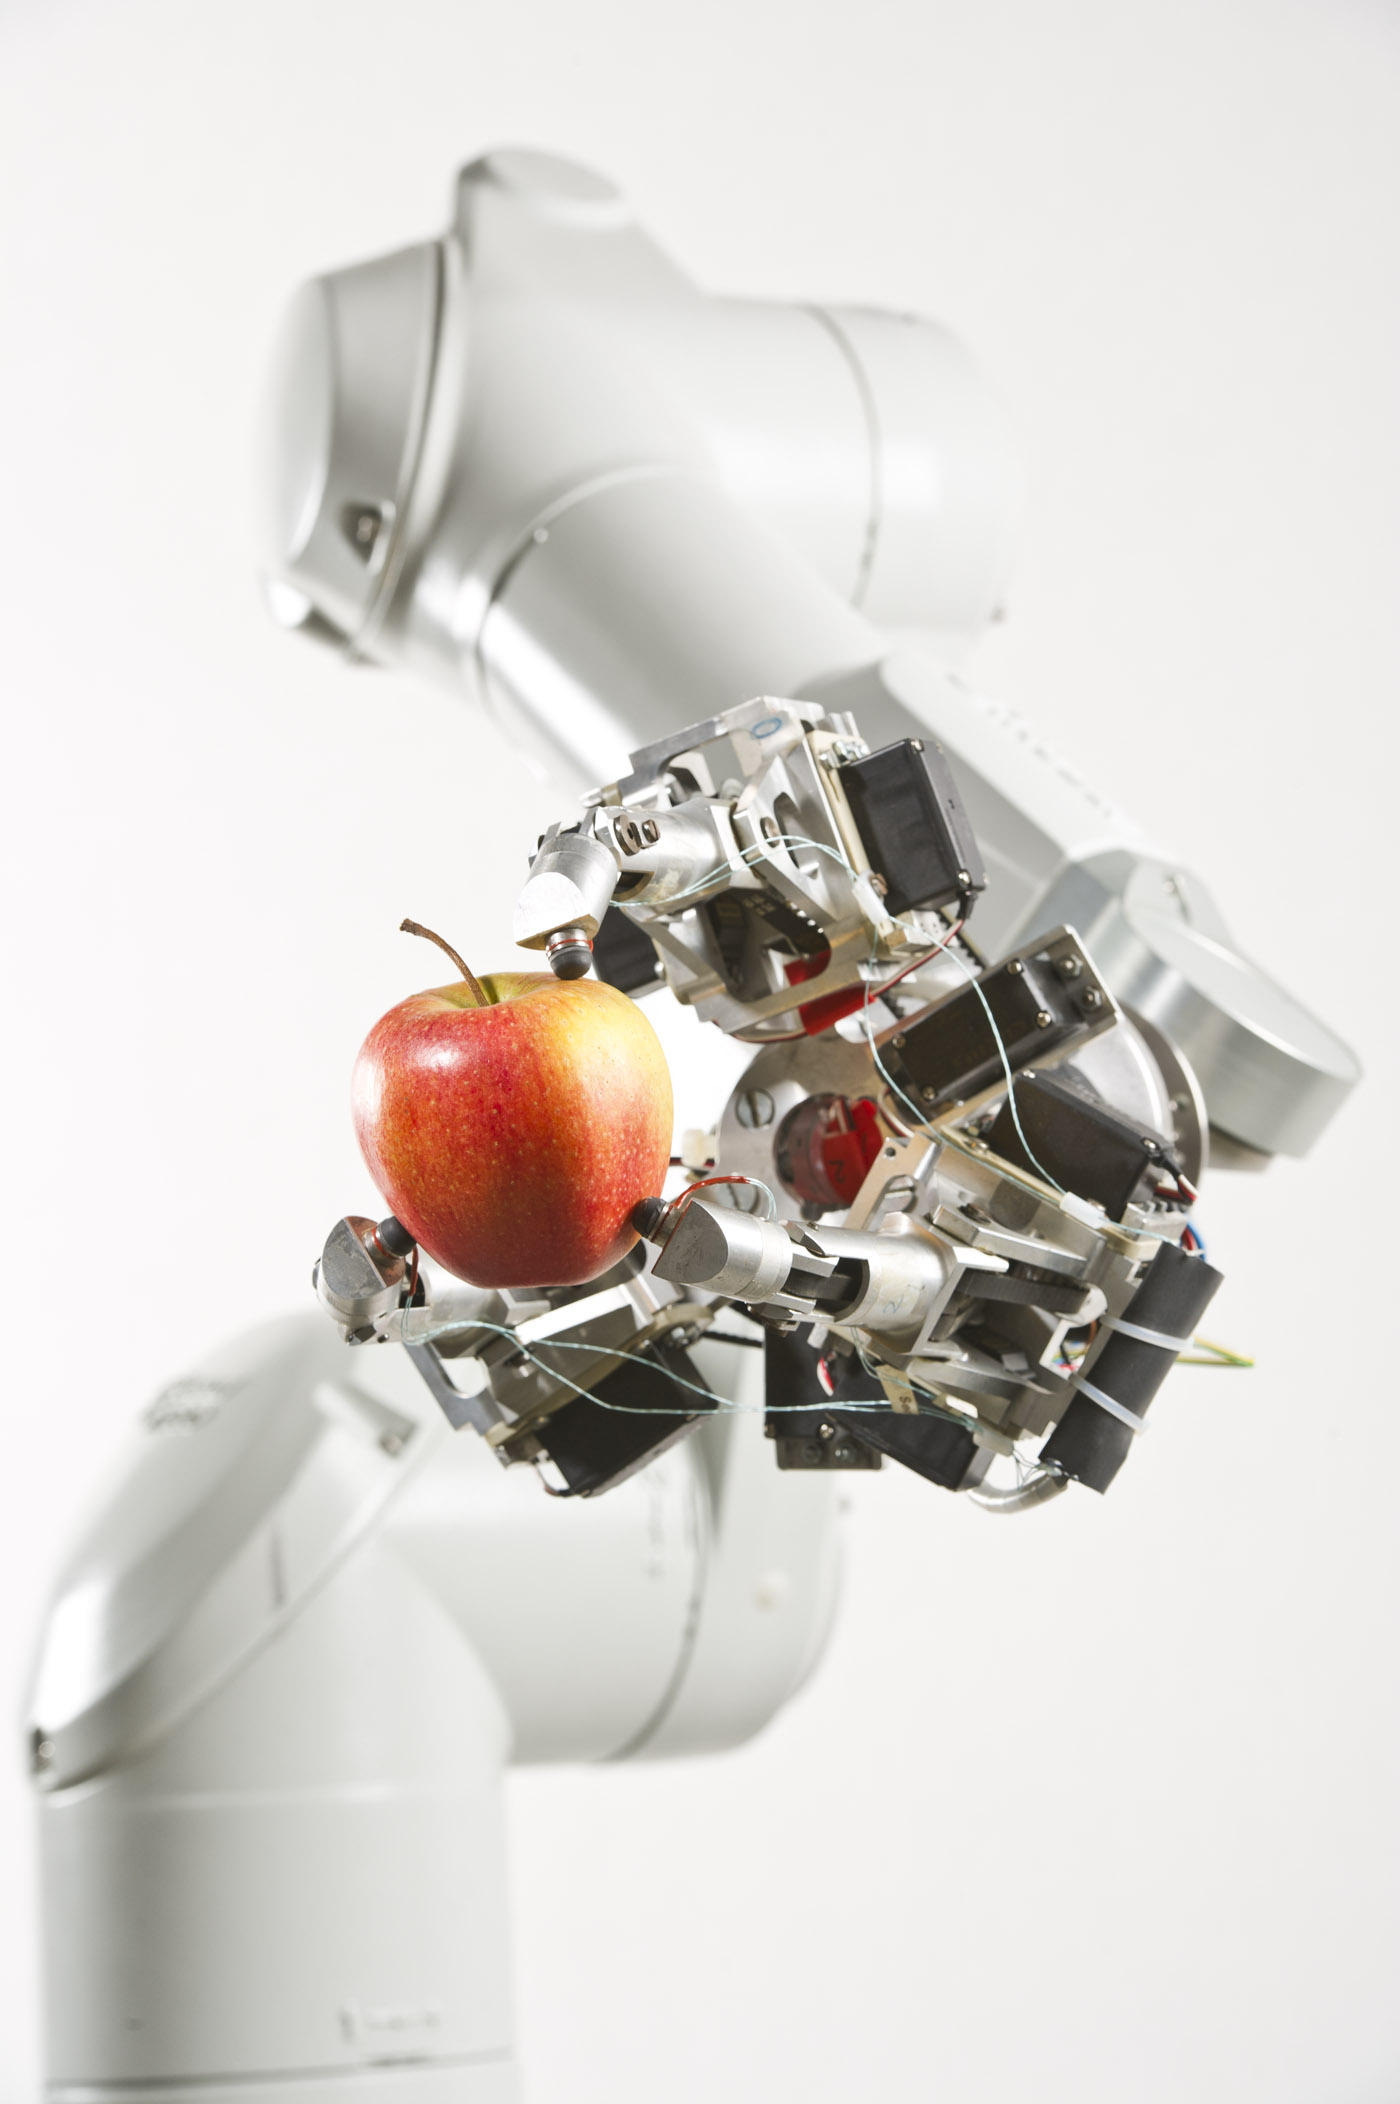
\includegraphics[height=\pictureheight]{Biomechgreifer.jpg}
		\subcaption{Roboterhand mit Apfel}
		\label{Bild_Beispiel_zwei_Bilder_links}
	\end{minipage}
%	
	\begin{minipage}[c]{.49\textwidth}
    		\centering
		
\includegraphics[height=\pictureheight]{LogoFAPS}
		\subcaption{FAPS-Logo}
		\label{Bild_Beispiel_zwei_Bilder_rechts}
	\end{minipage}
    	
    	\caption[Zwei Bilder nebeneinander]{Hier sind zwei Bilder zu sehen, welche nebeneinander angeordnet sind.}
	\label{Bild_Beispiel_zwei_Bilder}

\end{figure}

Auflistungen werden wie folgt gemacht:
\begin{itemize}
	\item Das wird der erste Stichpunkt \\ \vspace{-1cm}
	\item Der zweite Stichpunkt ist mit $\backslash\!vspace\left\{ -1cm \right\}$ in vertikaler Richtung verschoben \\ \vspace{-1cm}
\end{itemize}